\documentclass[11pt,a4paper]{article}

\usepackage[english,brazilian]{babel}
\usepackage{fontspec}
\defaultfontfeatures{Ligatures=TeX,Scale=MatchLowercase}
\usepackage[a4paper,top=2.35cm,bottom=2.35cm,left=2.55cm,right=2.55cm,headheight=15pt]{geometry}
\usepackage{microtype}
\usepackage{setspace}
\setstretch{1.06}
\setlength{\parindent}{1.15cm}
\setlength{\parskip}{0pt}
\setlength{\emergencystretch}{3em}

\usepackage{amsmath,amssymb,mathtools}
\usepackage{booktabs,array,tabularx}
\usepackage{caption}
\captionsetup{font=small,labelfont=bf,justification=justified,singlelinecheck=false}
\captionsetup[table]{position=top,skip=5pt}
\captionsetup[figure]{position=bottom,skip=6pt}
\usepackage{float,placeins}
\usepackage{enumitem}
\setlist{itemsep=2pt,topsep=4pt}
\usepackage{xcolor}
\definecolor{softblue}{HTML}{EFF5FA}
\definecolor{ruleblue}{HTML}{416A8A}
\definecolor{softred}{HTML}{FCEFEF}
\definecolor{softgreen}{HTML}{EDF7F0}
\usepackage{tikz}
\usetikzlibrary{arrows.meta,positioning,calc}
\usepackage{xurl}
\usepackage{fancyhdr}
\pagestyle{fancy}
\fancyhf{}
\fancyhead[L]{\small Validação técnica de grafos de comportamento}
\fancyhead[R]{\small Queiroz}
\fancyfoot[C]{\thepage}
\renewcommand{\headrulewidth}{0.3pt}

\usepackage[round,authoryear]{natbib}
\usepackage[unicode=true,pdfencoding=auto,psdextra]{hyperref}
\hypersetup{
  colorlinks=true,
  linkcolor=ruleblue,
  urlcolor=ruleblue,
  citecolor=ruleblue,
  pdftitle={Validação técnica da autoria de grafos de comportamento assistida por agentes de LLM},
  pdfauthor={João Carlos Queiroz},
  pdfsubject={Validação de caminhos corretos, ramos buggy, dicas, transporte e montagem GraphForge},
  pdfkeywords={sistemas tutores inteligentes; grafos de comportamento; CTAT; LLM; GraphForge; validação}
}
\usepackage{bookmark}

\newcolumntype{Y}{>{\raggedright\arraybackslash}X}
\newcolumntype{P}[1]{>{\raggedright\arraybackslash}p{#1}}
\newcolumntype{C}[1]{>{\centering\arraybackslash}p{#1}}
\newcolumntype{R}[1]{>{\raggedleft\arraybackslash}p{#1}}
\newcommand{\Rthreea}{\ensuremath{R_{3a,\mathrm{concreto}}}}
\newcommand{\Rthreeb}{\ensuremath{R_{3b,\mathrm{valor}}}}
\newcommand{\Cthreec}{\ensuremath{C_{3c,\mathrm{estrito}}}}
\newcommand{\ITT}{ITT}
\DeclareMathOperator{\LCS}{LCS}
\pdfstringdefDisableCommands{\def\Rthreea{R3a}\def\Rthreeb{R3b}\def\Cthreec{C3c}\def\ITT{ITT}}
\setcounter{secnumdepth}{2}

\begin{document}
\selectlanguage{brazilian}
\title{\bfseries Validação técnica da autoria de grafos de comportamento assistida por agentes de LLM}
\author{João Carlos Queiroz\\\small EducaOFF\\\small \href{mailto:contato@educaoff.com.br}{contato@educaoff.com.br}}
\date{}

\maketitle

\begin{abstract}
Este estudo avalia tecnicamente o processo de autoria de grafos de comportamento da EducaOFF, no qual três agentes de linguagem propõem caminhos corretos, erros com remediações e cadeias de dicas, enquanto o GraphForge monta a estrutura final. A análise principal utilizou 24 exercícios de frações na reta numérica, distribuídos em seis estados de quatro problemas e três réplicas, com o código implantado congelado e as referências CTAT isoladas até o fechamento das saídas. Dezessete dos 18 estados foram concluídos. O agente 3a apresentou recall concreto ordenado de 0 e correspondência exata da resposta final de 0,111 (IC95\% 0,028--0,222). O 3b recuperou 0,176 (0,113--0,242) dos valores errados únicos registrados na referência. No braço de capacidade do 3c, o sucesso estrito por problema foi 0,278 (0,167--0,403), a validade estrita condicional das cadeias foi 0,382 (0,257--0,507) e a taxa de vazamento literal da resposta foi 0,226 (0,172--0,285). O extrator reteve 22,1\% dos itens do 3a, 86,0\% dos erros do 3b e 82,9\% das dicas do 3c, mas eliminou \path{problemId} em todos os fluxos; a política operacional também omitiu o 3c nos 17 estados completos. O GraphForge reproduziu 34/34 pares de artefatos de forma idêntica. Um painel auxiliar de LLMs apresentou efeito teto e sensibilidade limitada, não oferecendo validação pedagógica independente. Os resultados sustentam uma validação técnica parcial: a montagem é reprodutível, mas há fragilidades de conteúdo, segurança e rastreabilidade que impedem recomendar uso autônomo. Eles não demonstram equivalência a especialistas nem eficácia educacional.

\smallskip\noindent\textbf{Palavras-chave:} sistemas tutores inteligentes; grafos de comportamento; CTAT; agentes de LLM; example-tracing; dicas; validação técnica.
\end{abstract}

\begin{otherlanguage}{english}
\renewcommand{\abstractname}{Abstract}
\begin{abstract}
This study technically evaluates EducaOFF's behavior-graph authoring process, in which three language-model agents propose correct paths, errors with remediation, and hint chains, while GraphForge assembles the final structure. The main analysis used 24 fraction number-line exercises arranged in six four-problem states and three replications, with the deployed code frozen and CTAT references isolated until outputs were closed. Seventeen of 18 states were completed. Agent 3a achieved an ordered concrete recall of 0 and an exact final-answer match of 0.111 (95\% CI 0.028--0.222). Agent 3b recovered 0.176 (0.113--0.242) of the unique wrong values recorded in the reference. In Agent 3c's capacity arm, strict success per problem was 0.278 (0.167--0.403), conditional strict validity among emitted chains was 0.382 (0.257--0.507), and literal answer leakage was 0.226 (0.172--0.285). The extractor retained 22.1\% of Agent 3a items, 86.0\% of Agent 3b errors, and 82.9\% of Agent 3c hints, but removed \path{problemId} from every flow; the operational policy also omitted Agent 3c in all 17 completed states. GraphForge reproduced 34/34 artifact pairs identically. An auxiliary LLM panel showed a ceiling effect and limited sensitivity, providing no independent pedagogical validation. The findings support partial technical validation: assembly is reproducible, but weaknesses in content, safety, and traceability preclude recommending autonomous use. They do not establish equivalence to experts or educational effectiveness.

\smallskip\noindent\textbf{Keywords:} intelligent tutoring systems; behavior graphs; CTAT; LLM agents; example tracing; hints; technical validation.
\end{abstract}
\end{otherlanguage}


\section{Introdução}

Tutores do paradigma \emph{example tracing} interpretam cada ação do estudante em relação a caminhos previamente autorados. No CTAT (Cognitive Tutor Authoring Tools), esses caminhos são registrados em grafos de comportamento que ligam estados, ações corretas, erros previstos, feedback e dicas \citep{aleven2009,aleven2016}. A utilidade do tutor depende, portanto, de mais do que uma topologia válida: ele precisa representar resoluções executáveis, antecipar erros relevantes e oferecer intervenções adequadas. A literatura clássica sobre \emph{bugs} procedimentais mostra por que esse trabalho de autoria importa: muitos erros não são aleatórios, mas expressam regras sistemáticas que podem ser reconhecidas e tratadas \citep{brown1978,vanlehn1990}.

Na EducaOFF, parte dessa autoria é assistida por três agentes baseados em modelos de linguagem. O agente 3a propõe o caminho correto; o 3b propõe erros, diagnósticos e remediações; e o 3c propõe hesitações e cadeias de dicas. Esses agentes não escrevem, sozinhos, a topologia final. Um extrator reduz e reorganiza suas saídas, e o GraphForge monta nós, arestas, scaffolds e manifestos. Neste artigo, a expressão ``grafos produzidos pelos agentes'' é uma abreviação para esse \textbf{fluxo assistido}: conteúdo candidato dos agentes, transformação pelo extrator e montagem determinística. A distinção evita atribuir ao modelo de linguagem uma perda que ocorreu no transporte, ou atribuir ao montador um conteúdo inadequado recebido dos agentes.

\begin{figure}[H]
  \centering
  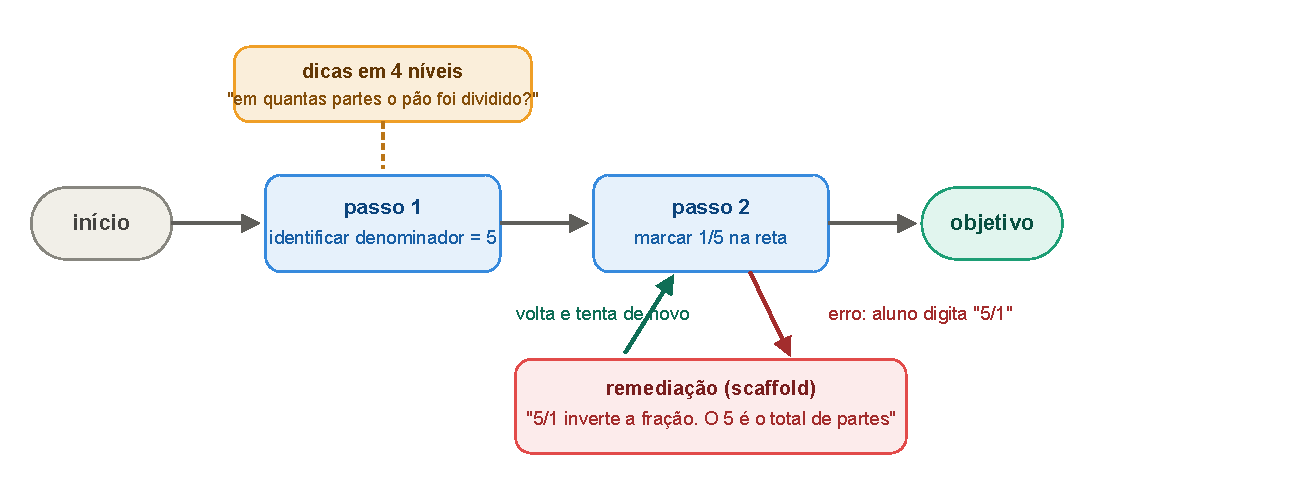
\includegraphics[width=0.94\linewidth]{../v6.0/figures/figura-01.pdf}
  \caption{Anatomia conceitual de um grafo de comportamento. O caminho horizontal representa uma resolução correta; o desvio inferior associa um erro previsto à remediação e ao retorno; o bloco superior representa uma cadeia progressiva de dicas. No fluxo estudado, os agentes propõem conteúdo e o GraphForge monta a topologia.}
  \label{fig:anatomia}
\end{figure}

Avaliar apenas se o arquivo final abre ou se o grafo é conectado seria insuficiente. Um artefato estruturalmente regular pode conter um caminho correto genérico demais para ser executado, ramos de erro sem localização, dicas que entregam a resposta ou itens pertencentes a exercícios diferentes depois de uma fusão sem proveniência. Por outro lado, comparar cada item gerado a um único grafo humano e chamar toda divergência de ``erro'' também seria inadequado: uma referência pode omitir estratégias e misconceptions plausíveis.

Neste trabalho, \textbf{validação técnica} significa reunir evidências separadas sobre seis camadas: (i) fidelidade da execução à rota auditada; (ii) conteúdo do caminho correto; (iii) cobertura, diagnóstico e remediação de comportamentos errôneos; (iv) completude e segurança dos scaffolds de dicas; (v) preservação de conteúdo e identidade durante o transporte; e (vi) integridade reprodutível da montagem. Essas camadas permitem responder onde o fluxo funciona e onde falha. Elas não estabelecem, por si só, validade pedagógica, equivalência a especialistas ou efeito sobre aprendizagem.

O estudo principal, denominado Campanha 4, foi desenhado depois que três campanhas exploratórias mostraram que uma bancada integrada não permitia localizar a origem das divergências. A Campanha 4 executa os agentes com o contrato multi-problema da rota legada implantada, preserva as saídas brutas antes da abertura das referências CTAT e mede separadamente geração, transporte e montagem. A pergunta central é: \emph{em que medida esse fluxo produz componentes observáveis de um grafo de comportamento concordantes com a referência CTAT, preservados no transporte e estruturalmente reproduzíveis?}

Essa pergunta é desdobrada em seis questões: concordância concreta do caminho correto; recuperação de erros previstos; qualidade formal e segurança das dicas; fidelidade de transporte; fidelidade da execução e reprodutibilidade da montagem; e contribuição de um painel cego de LLMs como evidência auxiliar. A contribuição do artigo é um instrumento auditável de diagnóstico por camada, acompanhado de uma avaliação empírica dos agentes como eles estavam configurados no fluxo legado da EducaOFF. Os detalhes históricos, matrizes completas, registros de modelos, incidentes, hashes e emendas ficam no suplemento técnico, preservando no texto principal apenas o necessário para avaliar método, resultados e alcance das conclusões.

\section{Fundamentação e modelo de validação}

\subsection{Objeto avaliado e fronteiras do fluxo}

Um grafo de conhecimento organiza habilidades e pré-requisitos no currículo; um grafo de comportamento representa estados e ações dentro de um exercício. O presente estudo trata exclusivamente do segundo objeto. A Figura~\ref{fig:pipeline} mostra as fronteiras observadas. O BRD, arquivo de referência autorado no CTAT, não alimentou os agentes nem o GraphForge: ele foi usado somente depois do fechamento das saídas, para calcular concordância. Agentes posteriores de adaptação do tutor e a rota atual \emph{tool-first} não fazem parte do experimento.

\begin{figure}[H]
\centering
\resizebox{\textwidth}{!}{%
\begin{tikzpicture}[
  node distance=6mm and 8mm,
  box/.style={draw=ruleblue,rounded corners=2pt,fill=softblue,align=center,minimum height=10mm,text width=26mm,font=\small},
  agent/.style={draw=ruleblue,rounded corners=2pt,fill=softgreen,align=center,minimum height=10mm,text width=25mm,font=\small},
  ref/.style={draw=red!55!black,dashed,rounded corners=2pt,fill=softred,align=center,minimum height=10mm,text width=28mm,font=\small},
  arrow/.style={-{Latex[length=2.2mm]},thick,draw=ruleblue},
  dasharrow/.style={-{Latex[length=2.2mm]},thick,dashed,draw=red!55!black}
]
\node[box] (state) {estado de autoria\\4 problemas-semente};
\node[agent,right=of state,yshift=13mm] (a) {Agente 3a\\traço correto};
\node[agent,right=of state] (b) {Agente 3b\\erros e remediação};
\node[agent,right=of state,yshift=-13mm] (c) {Agente 3c\\hesitações e dicas};
\node[box,right=12mm of b] (raw) {saídas brutas\\fechadas por hash};
\node[box,right=of raw] (extract) {extrator\\configuração};
\node[box,right=of extract] (forge) {GraphForge\\topologia e manifestos};
\node[ref,below=18mm of raw] (brd) {BRD CTAT\\referência de autoria};
\node[box,right=of brd] (metrics) {métricas por agente\\e por transporte};
\draw[arrow] (state) -- (a);
\draw[arrow] (state) -- (b);
\draw[arrow] (state) -- (c);
\draw[arrow] (a.east) -- (raw.west);
\draw[arrow] (b.east) -- (raw.west);
\draw[arrow] (c.east) -- (raw.west);
\draw[arrow] (raw) -- (extract);
\draw[arrow] (extract) -- (forge);
\draw[dasharrow] (brd) -- (metrics);
\draw[arrow] (raw.south) |- (metrics.west);
\draw[arrow] (forge.south) |- (metrics.east);
\node[font=\scriptsize,align=center,below=1mm of brd] {inacessível durante a autoria};
\end{tikzpicture}%
}
\caption{Fluxo efetivamente avaliado. A referência entra apenas na comparação, após o fechamento das saídas; por isso, concordância com o BRD e fidelidade de transporte podem ser analisadas sem contaminar a autoria.}
\label{fig:pipeline}
\end{figure}
\FloatBarrier

\subsection{Camadas de evidência e significado do BRD}

A unidade conceitual de validação é o processo que forma o grafo, não apenas o arquivo final. Como os agentes propõem componentes sem emitir uma topologia CTAT completa, uma comparação monolítica entre ``grafo do agente'' e BRD confundiria decisões dos agentes, do extrator e do GraphForge. A Tabela~\ref{tab:modelo} relaciona cada camada à evidência produzida e ao limite de sua interpretação. Não foi criado um escore global, porque uma média poderia compensar uma falha essencial --- por exemplo, bom formato textual não deveria apagar a perda de identidade do exercício.

\begin{table}[H]
\centering
\caption{Modelo de validação técnica em camadas.}
\label{tab:modelo}
\footnotesize
\setlength{\tabcolsep}{3pt}
\begin{tabularx}{\textwidth}{@{}P{2.35cm}P{3.0cm}Y Y@{}}
\toprule
Camada & Objeto observado & Evidência produzida & Limite da inferência \\
\midrule
Fidelidade de execução & código, configuração, entrada e política & correspondência com a rota legada congelada & não certifica versões futuras nem pesos remotos imutáveis \\
Caminho correto & saída do 3a e resposta final & instanciação concreta e concordância ordenada com ações do BRD & não julga sozinho a correção abstrata de templates genéricos \\
Ramos buggy & saída do 3b & cobertura por valor do catálogo de referência e campos remediativos & excedentes não são falsos automaticamente; localização CTAT exige estado/SAI \\
Scaffold de dicas & saída do 3c & quatro níveis, textos distintos e ausência de resposta literal & não mede aprendizagem nem adequação a estudantes reais \\
Transporte & configuração, grafo e manifesto & retenção de itens, campos e identidade de problema & preservar conteúdo não o torna pedagogicamente correto \\
Montagem & saídas GraphForge repetidas & identidade byte a byte e invariantes implementadas & determinismo não recupera dados descartados nem valida semântica \\
\bottomrule
\end{tabularx}
\end{table}

Os BRDs são adequados quando a pergunta é se o sistema reproduz elementos de STIs existentes. Eles registram decisões concretas de autoria e oferecem estados e triplas SAI (\emph{Selection--Action--Input}) que as saídas podem ou não recuperar. Contudo, há apenas um BRD por exercício. Sem autores independentes, não é possível separar a faceta ``exercício'' da faceta ``autor'' nem estimar uma faixa humano--humano, como exigiria uma análise de generalização entre facetas \citep{shavelson1991}. O BRD é, portanto, uma referência de concordância, não uma verdade pedagógica universal.

Essa cautela também é coerente com problemas conhecidos em avaliação de conteúdo gerado. Na geração automática de perguntas, por exemplo, os avaliadores e os protocolos podem divergir substancialmente \citep{amidei2018}. Esse resultado não prova variação entre autores CTAT; serve apenas como analogia metodológica para mostrar por que uma referência única não deve ser absolutizada. No presente estudo, cada item ficou em um de três territórios: interseção com o BRD, omissão em relação ao BRD ou excedente do sistema. A decomposição é inspirada na comparação assimétrica de características \citep{tversky1977}. Excedentes permanecem candidatos que exigem outra fonte de evidência.

Uma alegação futura de não inferioridade a especialistas precisaria de margem definida antes dos dados e de uma banda humano--humano observada. Testes de equivalência e não inferioridade não autorizam escolher a margem depois de olhar os resultados \citep{lakens2017,lakens2018}. Como essas condições não existem nas quatro campanhas, equivalência a especialistas é explicitamente não estimável.

\subsection{LLMs como juízes auxiliares}

LLMs podem aplicar rubricas em escala, mas não são árbitros externos neutros. Avaliadores automáticos podem reconhecer e favorecer produções de sua própria família \citep{panickssery2024}, e nem mesmo preferência humana agregada representa automaticamente todos os critérios de qualidade \citep{hosking2024}. Para reduzir dependência de uma única família, o painel deste estudo usa três famílias distintas da geradora, apresenta códigos opacos e não mostra o GraphForge. Mesmo assim, suas notas são auxiliares. Mutações sintéticas verificam se o painel reage a degradações óbvias; métricas determinísticas e limites de transporte mantêm prioridade.

\section{Método}

\subsection{Programa de pesquisa e desenho principal}

O projeto teve quatro campanhas sobre o mesmo corpus. As Campanhas 1 e 2 foram pilotos da bancada integrada; a segunda também variou o modelo gerador. A Campanha 3 construiu entradas sem ler o conteúdo comportamental do BRD e introduziu uma bateria de execução. Essas fases foram úteis para desenvolver o instrumento, mas não preservaram de forma comparável todas as saídas brutas dos três agentes. A Campanha 4 corrige essa lacuna ao observar diretamente agentes, extrator e GraphForge. A Tabela~\ref{tab:campanhas} resume as diferenças. Como entradas, runtimes, modelos auxiliares e estimandos mudaram, as campanhas não são réplicas e seus números não são combinados.

\begin{table}[H]
\centering
\caption{Função e comparabilidade das quatro campanhas.}
\label{tab:campanhas}
\footnotesize
\setlength{\tabcolsep}{3pt}
\begin{tabularx}{\textwidth}{@{}C{1.05cm}P{3.0cm}P{3.3cm}P{3.4cm}Y@{}}
\toprule
Fase & Objeto & Entrada & Desfecho central & Uso no artigo \\
\midrule
C1 & bancada integrada & envelopes derivados do BRD, com campos proibidos separados & cobertura por valor e integridade & piloto histórico \\
C2 & bancada integrada com quatro geradores & mesmo protocolo v1 & robustez exploratória da cobertura & contraste histórico entre braços \\
C3 & grafo integrado e executor analítico & interface e gabarito independentes do conteúdo do BRD & conformidade comportamental e ablações & evidência histórica integrada \\
C4 & agentes, extrator e GraphForge & contrato legado implantado, quatro problemas por estado & métricas por agente, transporte e montagem & estudo principal \\
\bottomrule
\end{tabularx}
\end{table}

O corpus \path{frac-numberline-6.17} contém 24 exercícios de localização de frações na reta numérica. Enunciados e respostas foram materializados a partir de uma chave independente derivada da interface, sem leitura dos BRDs. Os exercícios foram agrupados em seis estados de quatro problemas, cardinalidade esperada pela rota legada. Cada estado foi executado em três réplicas estocásticas, totalizando 18 unidades estado--réplica e 72 unidades exercício--réplica por agente. O provedor não expunha semente; ``réplica'' significa nova chamada com a mesma configuração.

A unidade principal foi o exercício. As réplicas foram primeiro agregadas dentro de cada um dos 24 exercícios e depois resumidas por média macro. Quatro exercícios compartilham a mesma chamada, criando dependência intra-batch. Por isso, além do bootstrap principal por exercício, foi calculada uma sensibilidade pós-hoc que reamostra os seis batches. Com apenas seis clusters, essa análise é descritiva e não resolve toda a incerteza.

As métricas e o protocolo inicial dos juízes foram congelados antes da primeira chamada paga. Três estados da primeira réplica foram usados como piloto e mantidos no conjunto final; o restante do plano foi formalizado depois desse piloto, sem inspeção das métricas de qualidade. A campanha é, assim, exploratória e auditável, mas não um pré-registro integral concluído antes de qualquer coleta.

\subsection{Fidelidade à implantação, agentes e isolamento da referência}

A execução utilizou uma cópia descartável da imagem de produção identificada pelo digest \path{sha256:15b29e8063099d40fc62899da2795db6e97d3e252e486315428a0690bb9abf5b}. O \emph{filesystem diff} estava vazio e os hashes dos agentes, do núcleo do pipeline, do GraphForge e do catálogo de misconceptions foram comparados com o manifesto. Como a imagem não contém rótulo VCS, o commit associado é fortemente corroborado, mas não provado. As chamadas não foram realizadas na VPS ativa; cache, fallback e retries internos foram desabilitados.

Os três agentes usaram \path{google/gemini-3.5-flash} via OpenRouter no tier \emph{balanced}. O 3a operou com temperatura 0,2 e limite de 16.000 tokens; o 3b, 0,7 e 24.000; o 3c, 0,4 e 16.000. Essas diferenças pertencem à configuração implantada, não são fatores experimentais. Os agentes 3a e 3b eram chamados em paralelo. O 3c seria chamado depois deles apenas quando a política operacional não o pulasse. Como essa política pulou o 3c em todos os estados completos, também foi executado um braço de \textbf{capacidade}, chamando o mesmo agente e prompt diretamente. Esse braço mostra o que o 3c consegue emitir; não representa sua contribuição efetiva ao fluxo operacional observado.

O processo de autoria não podia abrir BRDs, envelopes históricos ou resultados anteriores. A referência CTAT só foi aplicada depois da persistência das saídas brutas. O parser preservou estados e triplas SAI. A referência continha 96 ações corretas comparáveis e 192 ações buggy, das quais 110 passaram o filtro primário de conteúdo; sentinelas exatas e ações mecânicas foram excluídas por regra congelada.

\subsection{Desfechos e análise}

Os desfechos foram escolhidos para corresponder aos contratos reais dos agentes (Tabela~\ref{tab:estimandos}). A notação \ITT{} indica intenção de executar: falha de chamada, parse ou estado atômico entra como ausência ou zero, sem retry, reparo, fallback ou imputação. A análise restrita a estados completos é secundária.

\begin{table}[H]
\centering
\caption{Desfechos determinísticos do estudo principal.}
\label{tab:estimandos}
\footnotesize
\setlength{\tabcolsep}{3pt}
\begin{tabularx}{\textwidth}{@{}P{2.25cm}P{2.6cm}Y Y@{}}
\toprule
Componente & Desfecho & Definição operacional & Interpretação \\
\midrule
Caminho correto (3a) & \Rthreea & $\LCS(E,G_c)/|E|$, em que $E$ contém ações concretas ordenadas do BRD e $G_c$ resultados concretos gerados; placeholders recebem zero & instanciação e concordância concreta \\
Caminho correto (3a) & resposta final & igualdade exata após canonização & diagnóstico secundário de instanciação \\
Ramos buggy (3b) & \Rthreeb & recall de valores errados concretos únicos nas ações comparáveis do BRD & cobertura por valor da referência, não validade de excedentes \\
Localização (3b) & proxy ordinal & pareamento de número ordinal do passo e valor & sensibilidade; não equivale a estado ou SAI CTAT \\
Scaffold (3c) & \Cthreec & sucesso por problema se há passo elegível e todas as cadeias têm quatro níveis, tipos esperados, textos não vazios e distintos, sem resposta literal & qualidade operacional intrínseca \\
Transporte & retenção por item/campo & correspondência exata entre bruto, configuração, grafo e manifesto & preservação de informação \\
Montagem & determinismo & identidade byte a byte em duas execuções da mesma configuração & reprodutibilidade nos casos observados \\
\bottomrule
\end{tabularx}
\end{table}

O contrato do 3b não emite conjuntamente estado e SAI; portanto, o recall planejado por estado é não estimável. O número ordinal do passo foi mantido somente como sensibilidade, sem receber o nome de localização CTAT. Para o 3c, um passo é elegível quando contém \path{hesitation=true} ou dicas. Uma cadeia estrita exige níveis 1--4, tipos \path{conceptual}, \path{procedural}, \path{specific} e \path{bottom_out}, quatro textos distintos e ausência da resposta final literal.

Intervalos percentis de 95\% foram calculados por 20.000 reamostragens com reposição dos 24 exercícios, usando sementes fixas por métrica \citep{efron1993}. Eles descrevem estabilidade dentro do corpus e do mecanismo de reamostragem adotado, não uma população geral de STIs. A sensibilidade por batch preserva o agrupamento de quatro exercícios por chamada.

\subsection{Painel auxiliar e rastreabilidade}

O painel recebeu separadamente as 204 saídas principais observadas, 68 por agente. Os juízes foram \path{z-ai/glm-5.2}, \path{qwen/qwen3.7-plus} e \path{deepseek/deepseek-v4-pro}; o gerador pertencia à família Google. Cada juiz viu enunciado, resposta, KCs, passos independentes e a saída bruta, mas não identidade do agente, réplica, modelo, lote ou grafo montado. Cada papel possuía cinco dimensões em escala ordinal de 0 a 4. A mediana foi calculada quando ao menos dois julgamentos eram válidos; ausências não foram imputadas.

Seis exercícios predeterminados receberam uma mutação por papel, totalizando 18 saídas mutadas: contradição e remoção de passo no 3a; resposta errada substituída pelo gabarito e remoção parcial de diagnóstico/remediação no 3b; quatro dicas idênticas com entrega da resposta no 3c. Uma dimensão-alvo foi considerada sensível quando a nota caiu em pelo menos 80\% dos pares válidos. O alfa ordinal seguiu \citet{krippendorff2018}; o kappa nominal remonta a \citet{cohen1960}, e sua forma quadraticamente ponderada foi interpretada à luz de \citet{fleiss1973}. Quando havia uma única categoria observada, coeficientes corrigidos pelo acaso foram marcados como não estimáveis, em vez de tratados como concordância perfeita.

Estados, prompts, respostas, uso, custos, erros, configurações intermediárias, grafos e manifestos foram preservados com journal append-only e hashes SHA-256. O repositório também conserva lançamentos técnicos excluídos e erratas. Esses registros permitem auditar as decisões sem misturar tentativas inválidas ao painel final.

\section{Resultados}

\subsection{Execução do fluxo}

De 18 estados planejados, 17 foram concluídos (94,4\%). Na terceira réplica do batch 03, o provedor retornou respostas de 3a e 3b, mas o JSON de 3b era malformado. A resposta de 3a havia sido aceita pelo parser, porém o estado falhou atomicamente; o 3c não foi chamado. Não houve repetição nem reparo. Assim, 3a retornou 72 soluções identificáveis, mas 68 foram integradas. Para 3b e 3c, 68 unidades ficaram integráveis. As 72 unidades permanecem no denominador \ITT{}, que mede a efetividade do estado end-to-end, não a capacidade isolada do 3a.

\begin{table}[H]
\centering
\caption{Execução dos geradores na Campanha 4.}
\label{tab:execucao}
\footnotesize
\setlength{\tabcolsep}{2pt}
\begin{tabularx}{\textwidth}{@{}P{1.85cm}R{1.0cm}R{1.4cm}R{1.4cm}R{1.35cm}R{1.45cm}Y@{}}
\toprule
Componente & $N$ & Tokens entrada & Tokens saída & Custo (US\$) & Latência mediana & Resultado \\
\midrule
Agente 3a & 18 & 42.540 & 36.254 & 0,3901 & 11,47 s & 18 respostas; 17 estados integrados \\
Agente 3b & 18 & 53.268 & 87.248 & 0,8651 & 30,22 s & uma resposta malformada \\
Agente 3c --- capacidade & 17 & 49.607 & 69.372 & 0,6988 & 23,46 s & braço forçado; não chamado no estado falho \\
\midrule
Total & 53 & 145.415 & 192.874 & 1,9540 & 23,22 s & 52 respostas aceitas; 51 integradas \\
\bottomrule
\end{tabularx}
\begin{minipage}{\textwidth}\scriptsize\emph{Nota.} O custo total de US\$ 1,9540 inclui o braço forçado de capacidade do 3c. Ele é custo do experimento analítico, não custo do fluxo operacional observado, que pulou o 3c nos 17 estados completos.\end{minipage}
\end{table}

\subsection{Qualidade dos componentes autorados}

A Tabela~\ref{tab:diretas} apresenta as métricas diretas. Elas têm denominadores e significados diferentes e, por isso, não foram convertidas em uma nota única.

\begin{table}[H]
\centering
\caption{Métricas diretas dos agentes, sem escore composto.}
\label{tab:diretas}
\footnotesize
\setlength{\tabcolsep}{2pt}
\begin{tabularx}{\textwidth}{@{}C{1.05cm}Y C{1.65cm}C{1.75cm}P{3.45cm}@{}}
\toprule
Agente & Métrica & Estimativa & IC95\% bootstrap & Denominador/estatuto \\
\midrule
3a & Recall concreto ordenado \ITT{} & 0,000 & [0,000; 0,000] & 24 exercícios; 72 unidades \ITT{} \\
3a & Resposta final exata \ITT{} & 0,111 & [0,028; 0,222] & 24 exercícios; 72 unidades \ITT{} \\
3a & Resultados genéricos integrados & 1,000 & [1,000; 1,000] & 68 saídas pontuáveis \\
3b & Recall de valores errados únicos \ITT{} & 0,176 & [0,113; 0,242] & 24 exercícios; 72 unidades \ITT{} \\
3b & Recall nos estados completos & 0,190 & [0,124; 0,260] & 68 saídas observadas \\
3b & Proxy ordinal passo--valor \ITT{} & 0,060 & [0,023; 0,105] & sensibilidade; não é estado CTAT \\
3c & Sucesso estrito por problema \ITT{} & 0,278 & [0,167; 0,403] & braço de capacidade; 72 unidades \\
3c & Sucesso estrito, estados completos & 0,299 & [0,188; 0,424] & braço de capacidade; 68 saídas \\
3c & Completude 1--4 condicional & 1,000 & [1,000; 1,000] & 82 passos elegíveis \\
3c & Validade estrita condicional & 0,382 & [0,257; 0,507] & média macro entre cadeias emitidas \\
3c & Vazamento literal da resposta & 0,226 & [0,172; 0,285] & média macro entre dicas emitidas \\
\bottomrule
\end{tabularx}
\end{table}

Na sensibilidade que reamostrou os seis batches, o intervalo do acerto final do 3a ampliou-se para [0,000; 0,333]. Os intervalos do recall do 3b e do sucesso estrito do 3c foram [0,117; 0,244] e [0,153; 0,444]. O ponto central não mudou, mas a precisão do 3a era menor quando a chamada compartilhada era respeitada.

\paragraph{Caminho correto.} Todos os resultados intermediários do 3a continham placeholders como \texttt{\{A\}}, \texttt{\{B\}} e \texttt{\{C\}}, porque o próprio prompt pedia uma solução genérica. Por isso, a LCS concreta foi zero em todas as unidades. O resultado não demonstra que as relações abstratas estavam matematicamente erradas; demonstra que o contrato não entregava um traço concretamente executável. A correspondência exata da resposta final, 11,1\%, reforça que faltava uma etapa confiável de instanciação antes do uso no tutor.

\paragraph{Ramos buggy.} O 3b emitiu 136 erros concretos; nenhum tinha \path{wrongAnswer} igual à resposta correta. O agente recuperou 17,6\% dos valores errados únicos registrados no BRD sob \ITT{} e 19,0\% nos estados completos. Esse complemento não é uma taxa de erro do agente, pois o BRD pode omitir erros plausíveis. O que os dados mostram é baixa cobertura do catálogo específico e ausência de identidade estado/SAI para localizar os ramos com a precisão usada pelo CTAT.

\paragraph{Dicas.} No braço de capacidade, 82 passos elegíveis continham 328 dicas. Todas as cadeias tinham quatro níveis, mas apenas 32 satisfizeram simultaneamente os critérios estritos. Setenta e cinco mensagens continham literalmente a resposta final. As taxas agrupadas por item foram 39,0\% de cadeias estritas e 22,9\% de vazamento, próximas das médias macro da tabela. Assim, completar quatro níveis não garante progressão, distinção nem segurança. Além disso, a política operacional pulou o 3c em todos os 17 estados completos, de modo que nenhuma dessas dicas seguiria pelo fluxo observado sem o braço forçado.

\subsection{Transporte e montagem}

As perdas entre a saída bruta e o artefato final foram materialmente diferentes entre agentes (Tabela~\ref{tab:transporte}). O \path{problemId} desapareceu nos três fluxos, o que impede atribuir com segurança cada item ao exercício de origem depois da fusão multi-problema.

\begin{table}[H]
\centering
\caption{Retenção da saída bruta ao artefato de destino.}
\label{tab:transporte}
\footnotesize
\setlength{\tabcolsep}{3pt}
\begin{tabularx}{\textwidth}{@{}P{1.45cm}R{1.0cm}R{1.05cm}R{1.2cm}C{1.55cm}Y@{}}
\toprule
Agente & Bruto & Config. & Destino & Retenção & Perdas e campos críticos \\
\midrule
3a & 272 & 60 & 60 nós & 22,1\% & 212 itens truncados; ação e KC chegam aos nós, mas resultado e índice original não; \path{problemId} é descartado \\
3b & 136 & 117 & 117 erros & 86,0\% & 19 itens perdidos; identidade, localização e pergunta diagnóstica não chegam à configuração \\
3c, capacidade & 328 & 272 & 272 dicas & 82,9\% & nível, tipo e \path{problemId} são perdidos; textos ficam apenas no manifesto de slots \\
3c, operacional & 328\textsuperscript{a} & 0 & 0 & 0,0\% & a política pulou o agente nos 17 estados completos \\
\bottomrule
\multicolumn{6}{@{}p{\dimexpr\textwidth-2\tabcolsep\relax}@{}}{\scriptsize\textsuperscript{a} Os 328 itens pertencem ao braço forçado de capacidade. A linha operacional aplica a decisão real de \emph{skip}; não indica que a produção ordinária tenha chamado o 3c.}
\end{tabularx}
\end{table}

No 3a, o extrator concatena soluções e retém um prefixo global antes do GraphForge. Para o 3b, a maior parte do registro reduzido chega ao grafo, mas campos úteis para diagnóstico e localização já foram eliminados. Para o 3c, os textos sobrevivem no manifesto, sem nível nem tipo, e não aparecem nos nós do grafo genérico. Portanto, as percentagens de retenção não devem ser lidas isoladamente: 82,9\% de textos preservados ainda podem ser pouco utilizáveis quando a estrutura semântica que os organiza foi descartada.

O GraphForge produziu artefatos byte a byte idênticos em 34/34 pares de reexecução, cobrindo as políticas operacional e de capacidade nos 17 estados completos. Esse é um resultado favorável e claro sobre o montador. Ao mesmo tempo, ele delimita o que o determinismo resolve: a mesma entrada sobrevivente gera o mesmo artefato; itens cortados ou campos ausentes não são reconstruídos.

\subsection{Painel auxiliar}

O painel final realizou 666 julgamentos primários e 102 reparos, totalizando 768 chamadas e custo contábil de US\$ 1,2432. Qwen e DeepSeek completaram 222/222 unidades cada. O GLM completou 157/222; 65 julgamentos permaneceram ausentes, dos quais 59 tinham \path{confidence} fora do intervalo local e seis apresentavam JSON malformado. Apesar disso, todas as 204 saídas principais mantiveram ao menos dois juízes válidos.

As medianas agregadas foram 4 em todas as 15 dimensões. Entre notas válidas, 2.746 de 2.755 foram iguais a 4 (99,67\%); por agente, as proporções foram 99,79\%, 99,67\% e 99,54\% para 3a, 3b e 3c. Dez dimensões usaram uma única categoria e, por isso, alfa e kappa corrigidos pelo acaso eram não estimáveis. Nas cinco dimensões variáveis, o alfa ordinal ficou entre $-0{,}0055$ e 0,3294. A concordância bruta muito alta refletiu sobretudo o teto, não capacidade discriminativa.

Nas mutações, o painel reagiu a contradição e remoção de passo do 3a, remediação vazia do 3b e repetição com vazamento no 3c. Não reduziu as duas dimensões-alvo relacionadas à substituição do erro pelo gabarito e à remoção parcial do diagnóstico do 3b. Assim, seis de oito gates passaram. O painel reconheceu algumas degradações grosseiras, mas suas notas absolutas não acompanham falhas determinísticas como baixo recall, perda de identidade e vazamento literal. Ele não sustenta aprovação automática dos grafos.

\subsection{Triangulação com as campanhas históricas}

As três campanhas anteriores são apresentadas de forma resumida, sem combinação estatística com a Campanha 4. Na Campanha 1, a completude conceitual por valor foi 0,376 (IC95\% 0,309--0,442), a concordância bruta média foi 0,396 e o kappa médio de Cohen foi 0,007. A matriz completa, corrigida, representa a soma de 72 matrizes exercício--réplica; suas 437 classificações não são observações independentes. Na Campanha 2, nenhum contraste primário de completude contra o baseline permaneceu significativo após o procedimento de \citet{holm1979}; solicitar mais candidatos aumentou cobertura potencial, mas também custo e carga de revisão. Na Campanha 3, o reconhecimento comportamental integrado de ações buggy foi 0,054 (0,016--0,095) no baseline, e nenhum braço completou traços corretos inteiros.

Esses valores não medem o mesmo objeto das métricas diretas da Campanha 4. Ainda assim, a direção geral é informativa: as fases históricas mostravam cobertura parcial e baixa conformidade no subsistema integrado; a fase principal localiza mecanismos compatíveis com esse quadro, como placeholders, recuperação limitada do catálogo e perdas de transporte. A Tabela~\ref{tab:sintese} apresenta apenas a síntese permitida.

\begin{table}[H]
\centering
\caption{Síntese das evidências sobre a qualidade do fluxo auditado.}
\label{tab:sintese}
\footnotesize
\setlength{\tabcolsep}{3pt}
\begin{tabularx}{\textwidth}{@{}P{2.6cm}P{5.1cm}Y@{}}
\toprule
Dimensão & Evidência observada & Implicação defensável \\
\midrule
Regularidade & 17/18 estados concluídos; 52 respostas aceitas e 51 integradas & o fluxo geralmente produz saídas processáveis, mas falhas atômicas ocorrem \\
Caminho correto & recall concreto 0; resposta final exata 0,111; placeholders em todas as saídas integradas & falta um traço concretamente executável ou um instanciador validado \\
Ramos buggy & recall por valor 0,176; localização estado/SAI não estimável & há candidatos úteis, mas cobertura e localização não justificam uso automático \\
Dicas & sucesso estrito 0,278; validade condicional 0,382; vazamento 0,226; 3c pulado operacionalmente & completude formal não garante segurança e o fluxo observado não transportou dicas \\
Rastreabilidade & retenção 22,1\%/86,0\%/82,9\%; \path{problemId} perdido em todos os fluxos & conteúdo não pode ser atribuído com segurança depois da fusão \\
Montagem & 34/34 pares idênticos & o montador é reprodutível nos casos testados, mas não corrige entradas ou perdas \\
Plausibilidade textual & teto de 2.746/2.755 notas e mutações sensíveis em 6/8 dimensões & evidência auxiliar pouco discriminativa \\
Uso do artefato & ausência de novos especialistas e de estudo com estudantes & papel justificável: rascunho assistivo com gates e revisão humana \\
\bottomrule
\end{tabularx}
\end{table}

\section{Discussão}

\subsection{Os agentes produzem bons grafos de comportamento?}

Os resultados permitem uma resposta direta, mas não binária. Em engenharia, o fluxo tem dois pontos fortes: normalmente retorna conteúdo processável e monta de maneira reproduzível. Esses atributos são necessários para uma ferramenta de autoria, porém não bastam para um bom grafo de comportamento. No núcleo pedagógico observável --- caminho correto concreto, erros localizados, dicas seguras e proveniência --- a evidência é desfavorável ou insuficiente.

O 3a ilustra por que a avaliação em camadas muda o diagnóstico. Seu prompt pede um template genérico, enquanto o tutor precisa de ações concretas. O recall zero não autoriza dizer que todo raciocínio abstrato está errado; mostra que a interface entre agente e sistema não produz diretamente o objeto que será executado. A baixa correspondência da resposta final indica que o problema não se resolve apenas tolerando placeholders. Antes da montagem, o sistema precisa decidir se quer um traço concreto ou um template e, no segundo caso, provar que o instanciador determinístico preserva correção e ordem.

No 3b, o baixo recall mede omissão em relação a um catálogo específico, não falsidade de todos os excedentes. Mesmo assim, uma ferramenta que reproduza um STI existente deveria recuperar parte maior dos erros registrados ou justificar a diferença. Mais grave para o uso automático é a falta de estado/SAI no contrato e a perda posterior de identidade e localização. Um erro plausível, mas desconectado do ponto em que ocorre, não forma um ramo buggy operacional confiável.

No 3c, todas as cadeias observadas tinham quatro níveis, mas a qualidade estrita foi muito menor e houve resposta literal em aproximadamente uma de cada cinco dicas. Esse contraste mostra o limite de validar apenas schema. Além disso, o agente foi pulado pela política real em todos os estados completos. A avaliação de capacidade revela um material que poderia ser aproveitado depois de filtragem; ela não deve ser confundida com evidência de que o grafo operacional recebeu scaffolds adequados.

O transporte atravessa os três diagnósticos. Quando \path{problemId}, nível, tipo, localização ou resultado desaparecem, conteúdo potencialmente útil perde função no grafo. A retenção de 86,0\% no 3b e 82,9\% no 3c parece alta até que se observe quais campos foram descartados. Inversamente, o determinismo do GraphForge é um resultado positivo que ajuda a isolar responsabilidade: as diferenças não nascem de uma montagem aleatória, e sim do conteúdo recebido e das regras fixas que o reduzem.

Com base nos critérios observados, os artefatos não estão prontos para autoria autônoma. Isso não equivale a afirmar que ``os grafos são ruins'' em todas as dimensões ou que nenhum item gerado é aproveitável. A conclusão mais precisa é que o fluxo gera \textbf{rascunhos assistivos} com componentes potencialmente úteis, mas não demonstrou selecionar, instanciar, localizar e transportar esses componentes com segurança suficiente para publicação sem revisão.

\subsection{O que o instrumento valida --- e o que ainda falta}

O instrumento sustenta validação técnica de componentes: reproduz a rota auditada, compara saídas fechadas a uma referência, verifica propriedades das dicas, acompanha perdas de campo e testa repetibilidade da montagem. Essa decomposição é útil tanto para corrigir a plataforma quanto para comparar versões futuras. Uma melhora no 3b, por exemplo, pode ser distinguida de uma simples mudança no limite de truncamento; uma melhora nas dicas pode ser separada de uma alteração na política que decide chamá-las.

O instrumento não valida integralmente a pedagogia do tutor. Um BRD de autor único não captura todas as estratégias ou misconceptions legítimas. Sem novos especialistas, não é possível julgar sistematicamente os excedentes nem estimar a variação normal entre autores. Sem estudantes, não se sabe se diagnósticos e dicas melhoram resolução ou aprendizagem. Por isso, a presente conclusão não deve ser estendida a equivalência humana, validade de construto pedagógico ou eficácia educacional.

Também não se estima uma proporção de ``grafos corretos''. Esse desfecho não foi definido antes da coleta e exigiria regras para combinar dimensões incomensuráveis. Um grafo pode ser estruturalmente válido e pedagogicamente incompleto, ou conter bons candidatos que foram mal transportados. Manter o perfil por camada torna a limitação visível e evita que uma média esconda falhas críticas.

\subsection{BRDs e construção de um benchmark multi-STI}

Usar BRDs criados por especialistas é legítimo quando a meta é medir concordância com tutores existentes. A referência contém decisões de autoria que um sistema substituto deveria, em alguma medida, reproduzir. A defesa metodológica depende de formular a alegação corretamente: ``o sistema recupera X\% do catálogo deste BRD'' é suportável; ``X\% do conhecimento pedagógico verdadeiro'' não é.

Outros STIs podem ser adicionados ao mesmo protocolo e transformá-lo em benchmark, desde que cada caso preserve enunciado, interface, resposta, grafo de referência e proveniência. STIs, domínios e autores devem ser tratados como clusters; passos internos não podem inflar artificialmente a amostra. O conjunto deve separar desenvolvimento e teste, documentar autoria e licença e incluir, para uma parte representativa, pelo menos dois especialistas cegos adicionais com adjudicação. Só então seria possível estimar concordância humano--humano e discutir uma margem de não inferioridade.

Essa expansão não exige que todos os BRDs sejam idênticos em granularidade. Exige que a heterogeneidade seja registrada e modelada. Métricas por camada podem permanecer comuns, enquanto filtros de ações mecânicas e regras de canonização são declarados por corpus. O benchmark resultante avaliaria generalização entre STIs, em vez de repetir 24 variações de um único template.

\subsection{Implicações de engenharia}

Os resultados sugerem cinco mudanças antes de uma nova campanha:

\begin{enumerate}
  \item \textbf{Definir o contrato do 3a.} Exigir valores concretos quando o destino for execução, ou introduzir um instanciador determinístico com testes de correção e ordem.
  \item \textbf{Preservar identidade CTAT.} Fazer o 3b emitir estado e SAI e manter \path{problemId}, localização, pergunta diagnóstica e remediação até o artefato final.
  \item \textbf{Representar dicas como estrutura.} Conservar nível e tipo, executar filtro determinístico de resposta literal e tornar a decisão de pular o 3c explícita e auditável.
  \item \textbf{Eliminar truncamento global.} Aplicar limites dentro de cada \path{problemId}, registrando contadores e motivos de descarte.
  \item \textbf{Manter gates separados.} Schema, concordância com referência, transporte, integridade estrutural e revisão pedagógica não devem ser fundidos em um único \emph{quality score}.
\end{enumerate}

Essas correções mudam o sistema estudado e exigem uma nova versão do experimento. Os resultados atuais devem permanecer como baseline, inclusive a falha observada e os campos perdidos. Uma nova rodada pode reutilizar o instrumento e o corpus, mas deve ser reportada como comparação entre versões, não como substituição silenciosa do resultado adverso.

\subsection{Ameaças à validade}

\paragraph{Construto.} As métricas cobrem partes do grafo, não um conceito único de qualidade. \Rthreea{} penaliza placeholders exigidos pelo prompt e mede instanciação concreta, não correção abstrata. \Rthreeb{} ignora estado porque o contrato não o emite. As métricas do 3c avaliam forma e vazamento, não aprendizagem. Determinismo e retenção também não equivalem a adequação pedagógica.

\paragraph{Validade interna.} Um estado falhou atomicamente, impondo zero ao 3a mesmo com resposta parseável. O braço do 3c foi forçado e não representa a política operacional. A execução ocorreu em cópia descartável da imagem, com ontologia local de leitura; uma verificação pós-hoc do quarto KC não preservou respostas HTTP brutas da VPS. A imagem identifica o estado implantado por digest, mas não possui rótulo VCS. As Campanhas 1--3 usaram bancadas adaptadas e não permitem atribuição retrospectiva por agente.

\paragraph{Validade estatística.} O corpus tem 24 exercícios de um mesmo template, e quatro compartilham cada chamada. O bootstrap por exercício não representa totalmente essa dependência; a sensibilidade por batch tem apenas seis clusters. Réplicas e passos não são novas unidades independentes. Os intervalos descrevem este corpus e não uma população definida de STIs.

\paragraph{Referência e validade externa.} Há um BRD por exercício e a proveniência autoral e a licença do corpus ainda precisam de documentação completa. O estudo cobre frações na reta numérica, uma rota legada e um modelo gerador principal. Ele não cobre a rota atual, outros domínios, níveis escolares, interfaces, autores ou dados de estudantes.

\paragraph{Painel e conflito de interesses.} A composição dos juízes mudou depois do protocolo inicial por custo, embora o lançamento final tenha reiniciado do zero. O GLM teve perdas seletivas, o painel apresentou teto e não foi calibrado com especialistas. O autor é responsável pela plataforma avaliada. Preservar resultados adversos, lançamentos excluídos, hashes e limites de alegação reduz, mas não elimina, risco de viés.

\section{Conclusão}

O fluxo auditado produz conteúdo geralmente processável e uma montagem GraphForge reprodutível, mas não demonstrou, em conjunto, caminho correto concretamente executável, cobertura e localização suficientes de ramos buggy, scaffolds seguros nem proveniência preservada. O 3a operou com um contrato genérico incompatível com a comparação concreta; o 3b recuperou aproximadamente um quinto dos valores errados da referência e não forneceu localização CTAT completa; o 3c completou quatro níveis, mas apresentou validade estrita limitada e vazamento literal, além de ser omitido pela política operacional. O extrator agravou esse quadro ao remover conteúdo e identidade de problema.

Assim, a resposta empiricamente defensável é que os grafos não estão validados para uso autônomo na versão estudada. Eles podem servir como rascunhos assistivos submetidos a gates automáticos e revisão humana. O resultado não declara que todo conteúdo gerado seja incorreto, nem que o BRD contenha todas as possibilidades pedagógicas. Ele estabelece onde há evidência favorável, onde há fragilidade e onde a informação ainda é insuficiente.

O instrumento está pronto para comparar uma versão corrigida do pipeline e pode ser estendido a outros STIs como benchmark. Para sustentar uma alegação mais forte, a próxima etapa deve combinar múltiplos domínios, proveniência regularizada, especialistas independentes e, em estudo posterior, dados de uso com estudantes. Até lá, concordância com BRDs, segurança de dicas, fidelidade de transporte e integridade estrutural devem permanecer como evidências complementares, não como um selo único de qualidade.

\section*{Disponibilidade de dados e código}

O pacote de replicação, incluindo código, protocolos, resultados brutos e derivados públicos, está disponível em \href{https://github.com/Joaoqueiroz-silva/sti-graph-validation}{github.com/Joaoqueiroz-silva/sti-graph-validation}. O resultado determinístico principal encontra-se em \path{resultados/campanha4-2026-07-15/campaign4-final-analysis-v2.1.json}, e o painel final em \path{resultados/campanha4-2026-07-15/judge-panel-v5/}. A redistribuição dos BRDs depende de regularização documental de autoria e licença; hashes e métricas não conferem essa permissão. O suplemento técnico descreve matrizes históricas, hashes, incidentes e emendas.

\section*{Declarações}

\textbf{Conflito de interesses.} O autor é fundador da EducaOFF, plataforma cujo subsistema foi avaliado.

\textbf{Ética.} O estudo não envolveu participantes humanos, dados pessoais ou dados de estudantes. Estudos futuros com especialistas ou estudantes deverão seguir a avaliação ética aplicável.

\textbf{Uso de inteligência artificial.} Modelos de linguagem são objeto do experimento e também apoiaram engenharia, auditoria e revisão do texto. As decisões metodológicas, a interpretação e a responsabilidade pelo conteúdo permanecem com o autor. Julgamentos automatizados não substituíram anotação humana independente.

\begin{thebibliography}{99}

\bibitem[Aleven et al.(2009)]{aleven2009}
Vincent Aleven, Bruce M. McLaren, Jonathan Sewall, and Kenneth R. Koedinger.
\newblock A new paradigm for intelligent tutoring systems: Example-tracing tutors.
\newblock \emph{International Journal of Artificial Intelligence in Education}, 19(2):105--154, 2009.
\newblock URL: \url{https://eric.ed.gov/?id=EJ902546}.

\bibitem[Aleven et al.(2016)]{aleven2016}
Vincent Aleven, Bruce M. McLaren, Jonathan Sewall, Martin van Velsen, Octav Popescu, Sandra Demi, Michael Ringenberg, and Kenneth R. Koedinger.
\newblock Example-tracing tutors: Intelligent tutor development for non-programmers.
\newblock \emph{International Journal of Artificial Intelligence in Education}, 26(1):224--269, 2016.
\newblock DOI: \url{https://doi.org/10.1007/s40593-015-0088-2}.

\bibitem[Amidei et al.(2018)]{amidei2018}
Jacopo Amidei, Paul Piwek, and Alistair Willis.
\newblock Evaluation methodologies in automatic question generation 2013--2018.
\newblock In \emph{Proceedings of the 27th International Conference on Computational Linguistics}, pages 3318--3329, Santa Fe, New Mexico, USA, 2018. Association for Computational Linguistics.
\newblock URL: \url{https://aclanthology.org/C18-1281/}.

\bibitem[Brown and Burton(1978)]{brown1978}
John Seely Brown and Richard R. Burton.
\newblock Diagnostic models for procedural bugs in basic mathematical skills.
\newblock \emph{Cognitive Science}, 2(2):155--192, 1978.
\newblock DOI: \url{https://doi.org/10.1207/s15516709cog0202_4}.

\bibitem[Cohen(1960)]{cohen1960}
Jacob Cohen.
\newblock A coefficient of agreement for nominal scales.
\newblock \emph{Educational and Psychological Measurement}, 20(1):37--46, 1960.
\newblock DOI: \url{https://doi.org/10.1177/001316446002000104}.

\bibitem[Efron and Tibshirani(1993)]{efron1993}
Bradley Efron and Robert J. Tibshirani.
\newblock \emph{An Introduction to the Bootstrap}.
\newblock Chapman \& Hall, New York, 1993. Monographs on Statistics and Applied Probability, volume 57. ISBN 978-0-412-04231-7.
\newblock URL: \url{https://www.routledge.com/An-Introduction-to-the-Bootstrap/Efron-Tibshirani/p/book/9780412042317}.

\bibitem[Fleiss and Cohen(1973)]{fleiss1973}
Joseph L. Fleiss and Jacob Cohen.
\newblock The equivalence of weighted kappa and the intraclass correlation coefficient as measures of reliability.
\newblock \emph{Educational and Psychological Measurement}, 33(3):613--619, 1973.
\newblock DOI: \url{https://doi.org/10.1177/001316447303300309}.

\bibitem[Holm(1979)]{holm1979}
Sture Holm.
\newblock A simple sequentially rejective multiple test procedure.
\newblock \emph{Scandinavian Journal of Statistics}, 6(2):65--70, 1979.
\newblock DOI: \url{https://doi.org/10.2307/4615733}.

\bibitem[Hosking et al.(2024)]{hosking2024}
Tom Hosking, Phil Blunsom, and Max Bartolo.
\newblock Human feedback is not gold standard.
\newblock In \emph{International Conference on Learning Representations}, 2024.
\newblock URL: \url{https://openreview.net/forum?id=7W3GLNImfS}.

\bibitem[Krippendorff(2018)]{krippendorff2018}
Klaus Krippendorff.
\newblock \emph{Content Analysis: An Introduction to Its Methodology}.
\newblock SAGE Publications, Thousand Oaks, California, fourth edition, 2018. ISBN 978-1-5063-9566-1.
\newblock URL: \url{https://www.sagepub.com/shop/buy-a-book/content-analysis-4-258450}.

\bibitem[Lakens(2017)]{lakens2017}
Dani\"el Lakens.
\newblock Equivalence tests: A practical primer for $t$ tests, correlations, and meta-analyses.
\newblock \emph{Social Psychological and Personality Science}, 8(4):355--362, 2017.
\newblock DOI: \url{https://doi.org/10.1177/1948550617697177}.

\bibitem[Lakens et al.(2018)]{lakens2018}
Dani\"el Lakens, Anne M. Scheel, and Peder M. Isager.
\newblock Equivalence testing for psychological research: A tutorial.
\newblock \emph{Advances in Methods and Practices in Psychological Science}, 1(2):259--269, 2018.
\newblock DOI: \url{https://doi.org/10.1177/2515245918770963}.

\bibitem[Panickssery et al.(2024)]{panickssery2024}
Arjun Panickssery, Samuel R. Bowman, and Shi Feng.
\newblock LLM evaluators recognize and favor their own generations.
\newblock In \emph{Advances in Neural Information Processing Systems}, volume 37, pages 68772--68802, 2024.
\newblock DOI: \url{https://doi.org/10.52202/079017-2197}.

\bibitem[Shavelson and Webb(1991)]{shavelson1991}
Richard J. Shavelson and Noreen M. Webb.
\newblock \emph{Generalizability Theory: A Primer}.
\newblock SAGE Publications, Newbury Park, California, 1991. ISBN 978-0-8039-3745-1.
\newblock URL: \url{https://www.sagepub.com/shop/buy-a-book/generalizability-theory-1-3375}.

\bibitem[Tversky(1977)]{tversky1977}
Amos Tversky.
\newblock Features of similarity.
\newblock \emph{Psychological Review}, 84(4):327--352, 1977.
\newblock DOI: \url{https://doi.org/10.1037/0033-295X.84.4.327}.

\bibitem[VanLehn(1990)]{vanlehn1990}
Kurt VanLehn.
\newblock \emph{Mind Bugs: The Origins of Procedural Misconceptions}.
\newblock MIT Press, Cambridge, Massachusetts, 1990. ISBN 978-0-262-22036-1.
\newblock URL: \url{https://mitpress.mit.edu/9780262220361/mind-bugs/}.

\end{thebibliography}


\end{document}
